\chapter{Results and discussion}

\section{False positive assignments have lower scores}

In the proteins we analysed, the theoretical positions of DBs are known. We call a fragment (and by extension, the whole variant) that contradicts the knowledge about DB positions a \emph{bad} fragment. We have evaluated our variant scoring metric on four different datasets (LYS, LIP, GENOVA, and BSA), separately on good and bad variants; the results are presented on \Cref{fig:scoring-metric}. A clear difference between the median variant score of the bad and the good variants can be seen.

\begin{figure}
  \centering
  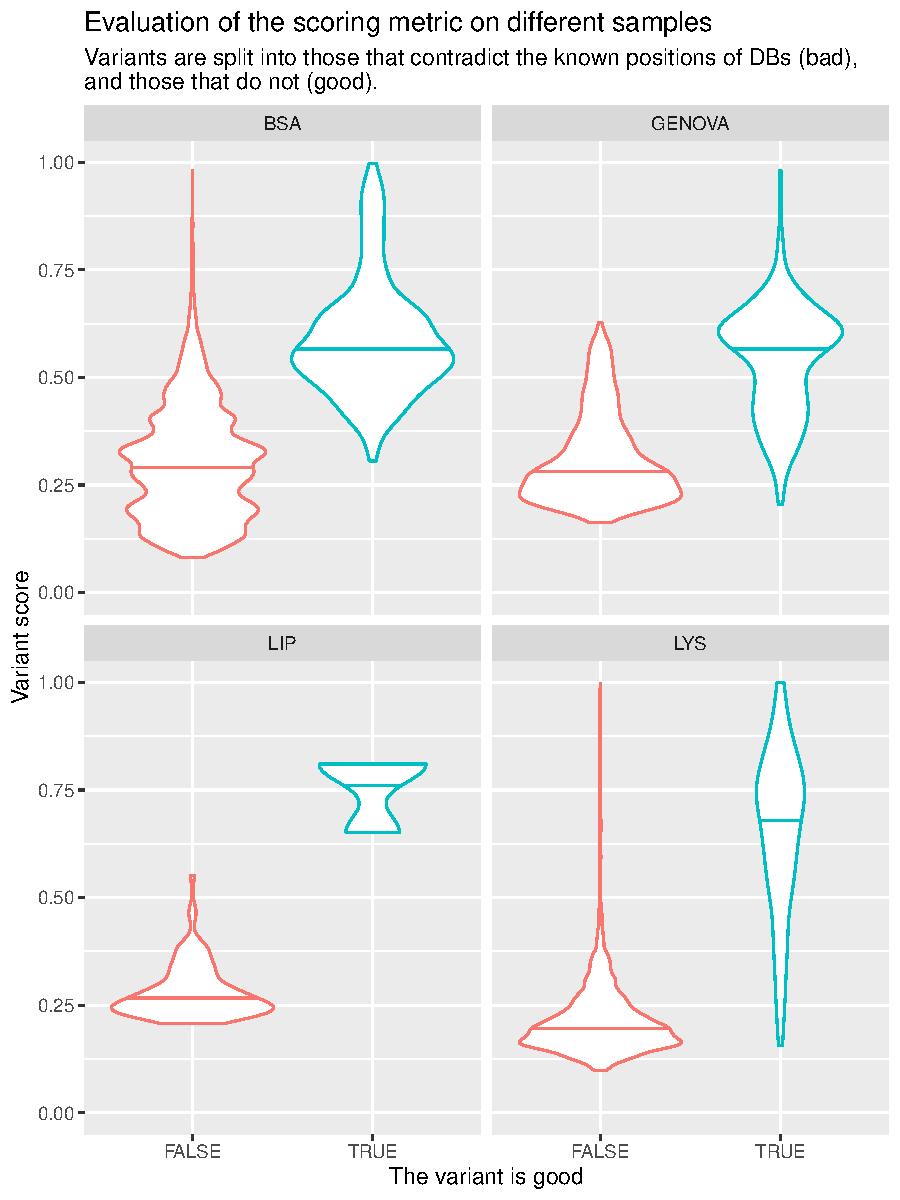
\includegraphics[width=1\linewidth]{img/scoring-metric-evaluation.pdf}
  \caption{Scoring metric evaluation on datasets from four different samples. Individual datapoints represent different assigned variants, that are grouped based on whether they contradict expert knowledge about DB positions. The boxplots illustrate that the separation is usually relatively good, but as we can see from the datapoints, there are still a lot of (in theory) nonexsting variants with a high score. This can partly be attributed to DB scrambling. The lack of data in the LIP sample is discussed in the text. (BSA = bovine serum albumin, LYS = lysosyme, LIP = lipase, GENOVA = an in-silico generated ovalbumin dataset)}\label{fig:scoring-metric}
\end{figure}

\section{Some DBs were successfully identified}

A complete DB analysis was performed on three proteins, namely LYS, LIP, and GENOVA\@. The analysis was initially run with vanilla settings. If there had been a strong evidence for a particular DB in the RAT data, it was deemed to be prone to generating false positive signals. Consequently, its weight has been adjusted to 0.1, or 0.8, depending on the strength of its RAT evidence, and the analysis was run again.

The results from the second run of the analysis can be seen on the following figures: \Cref{fig:lys} (LYS), \Cref{fig:lip} (LIP), and \Cref{fig:genova} (GENOVA). The top row shows data from RAT samples, the bottom shows data from AT samples, the left column shows the theoretical positions of the cysteine alkylations and disulfide bonds, and the right column shows the aggregated evidence. Alkylation evidence is illustrated by a border around the cysteine.

As is apparent from the images, Dibby generates a lot of false positive signal. However, the scoring and weighting of the evidence helps immensely, and some DBs are clearly identifiable; three in the LYS sample (of the four total DBs), one in the LIP sample (of the three total DBs), and one in the GENOVA sample (the only DB that is present).


\paragraph{Lysosyme} Three of the four DBs have been identified successfully (\Cref{fig:lys}). The last DB cysteine pair was seen only in 7 good fragments, compared for example to the 2,534 good fragments of the bond \((5, 126)\). In other words, its signal is very low in comparison with the other bonds. We are not sure what caused this stark disparity, and the causes should be more deeply investigated in the future. The evidence for the bond \((75, 93)\) is not as strong as for the other two, relative to the evidence for alkylations of the respective cysteines. The bond is objectively hard to identify, because there is no tryptic cleavage point between the cysteines. The fact that Dibby has been able to identify this bond foreshadows the power of its general assignment algorithm.

\begin{figure}
  \centering
  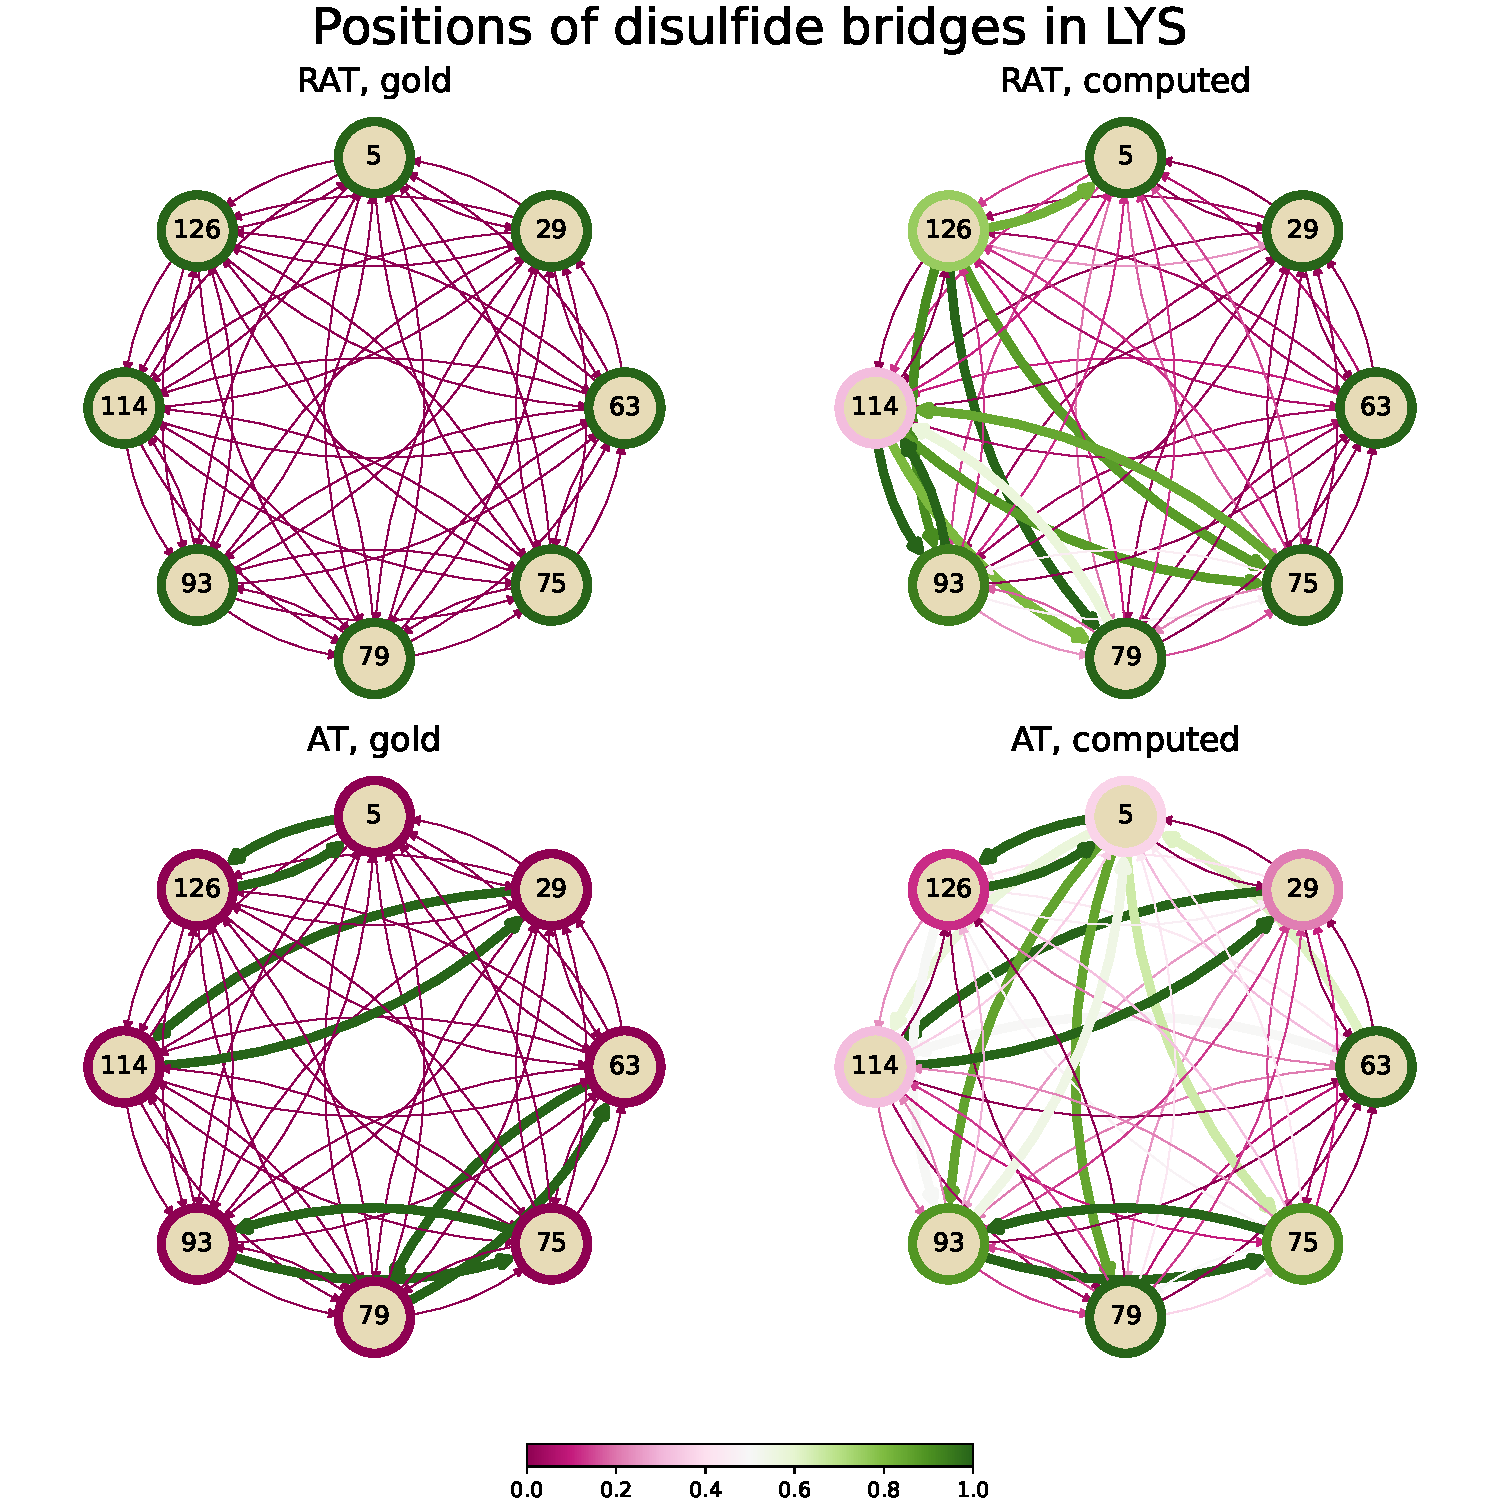
\includegraphics[width=1\linewidth]{img/lys.pdf}
  \caption{The evidence for positions of DBs and alkylations in lysosyme, weighted by variant score, and normalised. There are quite a few false positives, however, the bonds \((5, 126)\) and \((29, 114)\) are still clearly visible. We can safely ignore the other directed edges stemming from 5, because their scores are relatively low compared to \((5, 126)\), and also because they are not bidirectional --- that means that the supposed bond-partners are seen more commonly in other configurations. The presence of the bond \((75, 93)\) is not so clear-cut; we also have strong signals about the cysteines being alkylated. This varrants further investigation. Finally, the evidence for bond \((63, 79)\) is practically not present, and both cysteines were deemed as alkylated.}\label{fig:lys}
\end{figure}

\paragraph{Generated ovalbumin} Similarly to the lysosyme plots, some false positives had cropped up (\Cref{fig:lip}), though they did not manage to drown out the true evidence. The only present DB, \((72, 119)\), has been successfully identified. There are some directed edges coming into the cysteine 119, however; the algorithm and the scoring system should be finetuned so that similar false positives do not slip through the cracks, or at least do not provide such a strong signal.

\begin{figure}
  \centering
  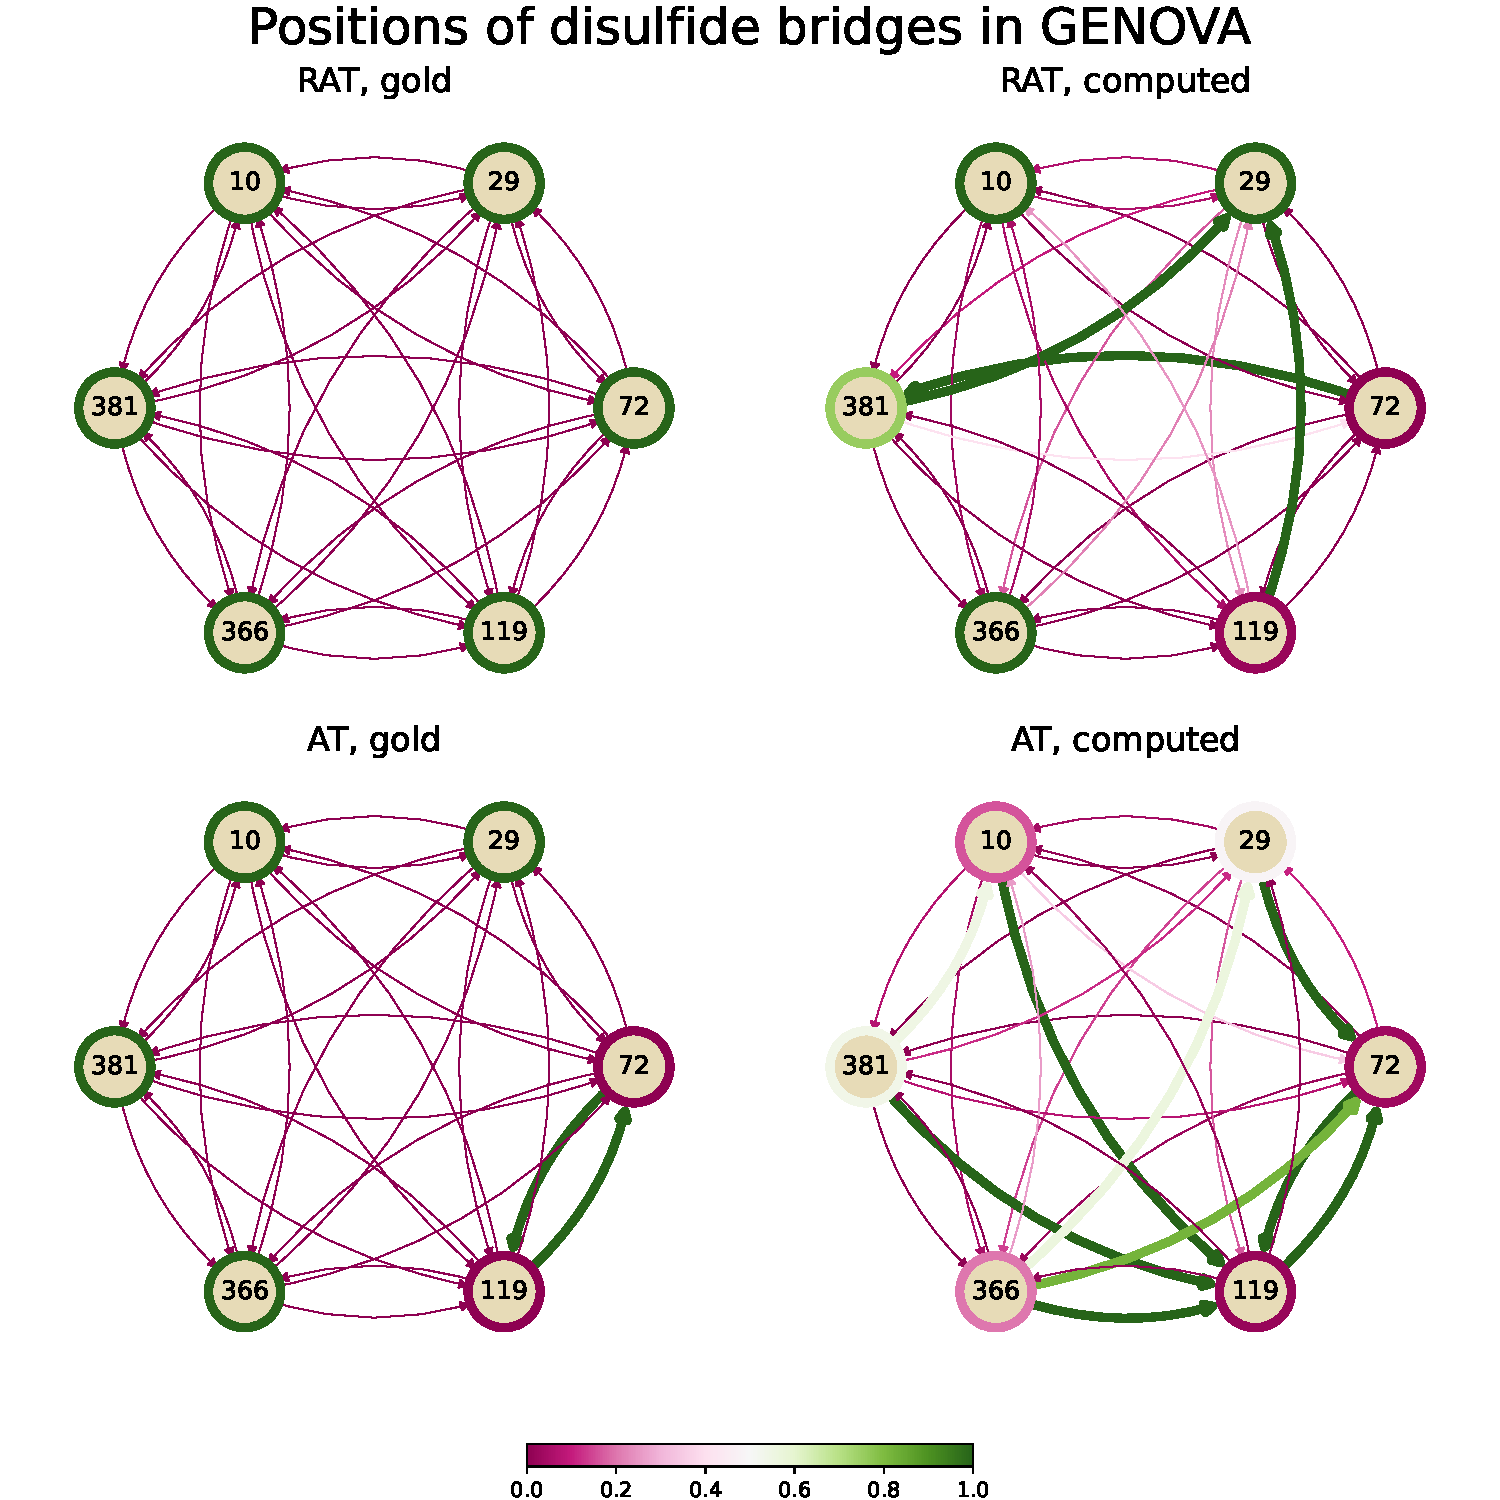
\includegraphics[width=1\linewidth]{img/genova.pdf}
  \caption{The evidence for positions of DBs and alkylations in in-silico generated ovalbumin, weighted by variant score, and normalised. Although there are some false positives, leading mainly to cysteine 119, the only confirmed bidirectional bond is the correct one: \((72, 119)\). }\label{fig:genova}
\end{figure}

\paragraph{Lipase} Only one of the three DBs has been identified in the LIP sample (\Cref{fig:lip}). Interestingly, we have identified exactly zero variants containing the cysteines 271 and 295, alkylated or otherwise. To test whether this had been caused by a problem in the data or the algorithm, we have ran a MSGF+~\cite{kim2014ms} analysis on the LIP samples (and later on the other samples as well); the comparison with results from Dibby is in \Cref{tbl:measurements}. We can see that even MSFG+, a state of the art proteomic database search tool, had problems with LIP data, suggesting an unknown issue occured during the sample preparation, rendering most of the LIP data unuseable.


% Please add the following required packages to your document preamble:
% \usepackage{booktabs}
% \usepackage{multirow}
\begin{table}[]
  \begin{tabular}{@{}llllll@{}}
    \toprule
    \multicolumn{1}{c}{\multirow{2}{*}[-0.25em]{Sample}} & \multirow{2}{*}[-0.25em]{Scans} & \multicolumn{1}{c}{\multirow{2}{*}[-0.2em]{\begin{tabular}[c]{@{}c@{}}MSGF+\\ Matches\end{tabular}}} & \multicolumn{3}{c}{Dibby matches}               \\ \cmidrule(l){4-6}
    \multicolumn{1}{c}{}                                 &                                 & \multicolumn{1}{c}{}                                                   & Simple                            & Total & DBs \\ \midrule
    LYS AT                                               & 12479                           & 411                                                                    & 463                               & 2240  & 3/4 \\
    LYS RAT                                              & 14517                           & 1216                                                                   & 2157                              & 2972  &     \\
    LIP AT                                               & 13579                           & 21                                                                     & 12                                & 67    & 1/3 \\
    LIP RAT                                              & 14177                           & 76                                                                     & 66                                & 131   &     \\
    GENOVA AT                                            & 1606                            &                                                                        & 855                               & 3257  & 1/1 \\
    GENOVA RAT                                           & 735                             &                                                                        & 770                               & 805   &     \\
    BSA AT                                               & 13856                           & 1495                                                                   & 1717                              & 48222 &     \\
    BSA RAT                                              & 14242                           & 1723                                                                   & 2684                              & 22133 &     \\ \bottomrule
  \end{tabular}

  \caption{Comparison of Dibby with MSGF+, a state of the art database search tool for proteomics. MSGF+ can only identify peptides that are not cross-linked, or ``simple'' peptides; for this reason, we list the number of Dibby's simple assignments in addition to the total number of its assignments. Generally, Dibby identifies a little bit more precursors than MSGF+, most of which are probably false positives. There are close to 0 false negatives, however. There is clearly a problem with lipase data; MSGF+ identified 16 times more precursors in the LYS RAT sample, although the number of measured scans in the mgf file is comparable with LIP RAT.}\label{tbl:measurements}
\end{table}

\begin{figure}
  \centering
  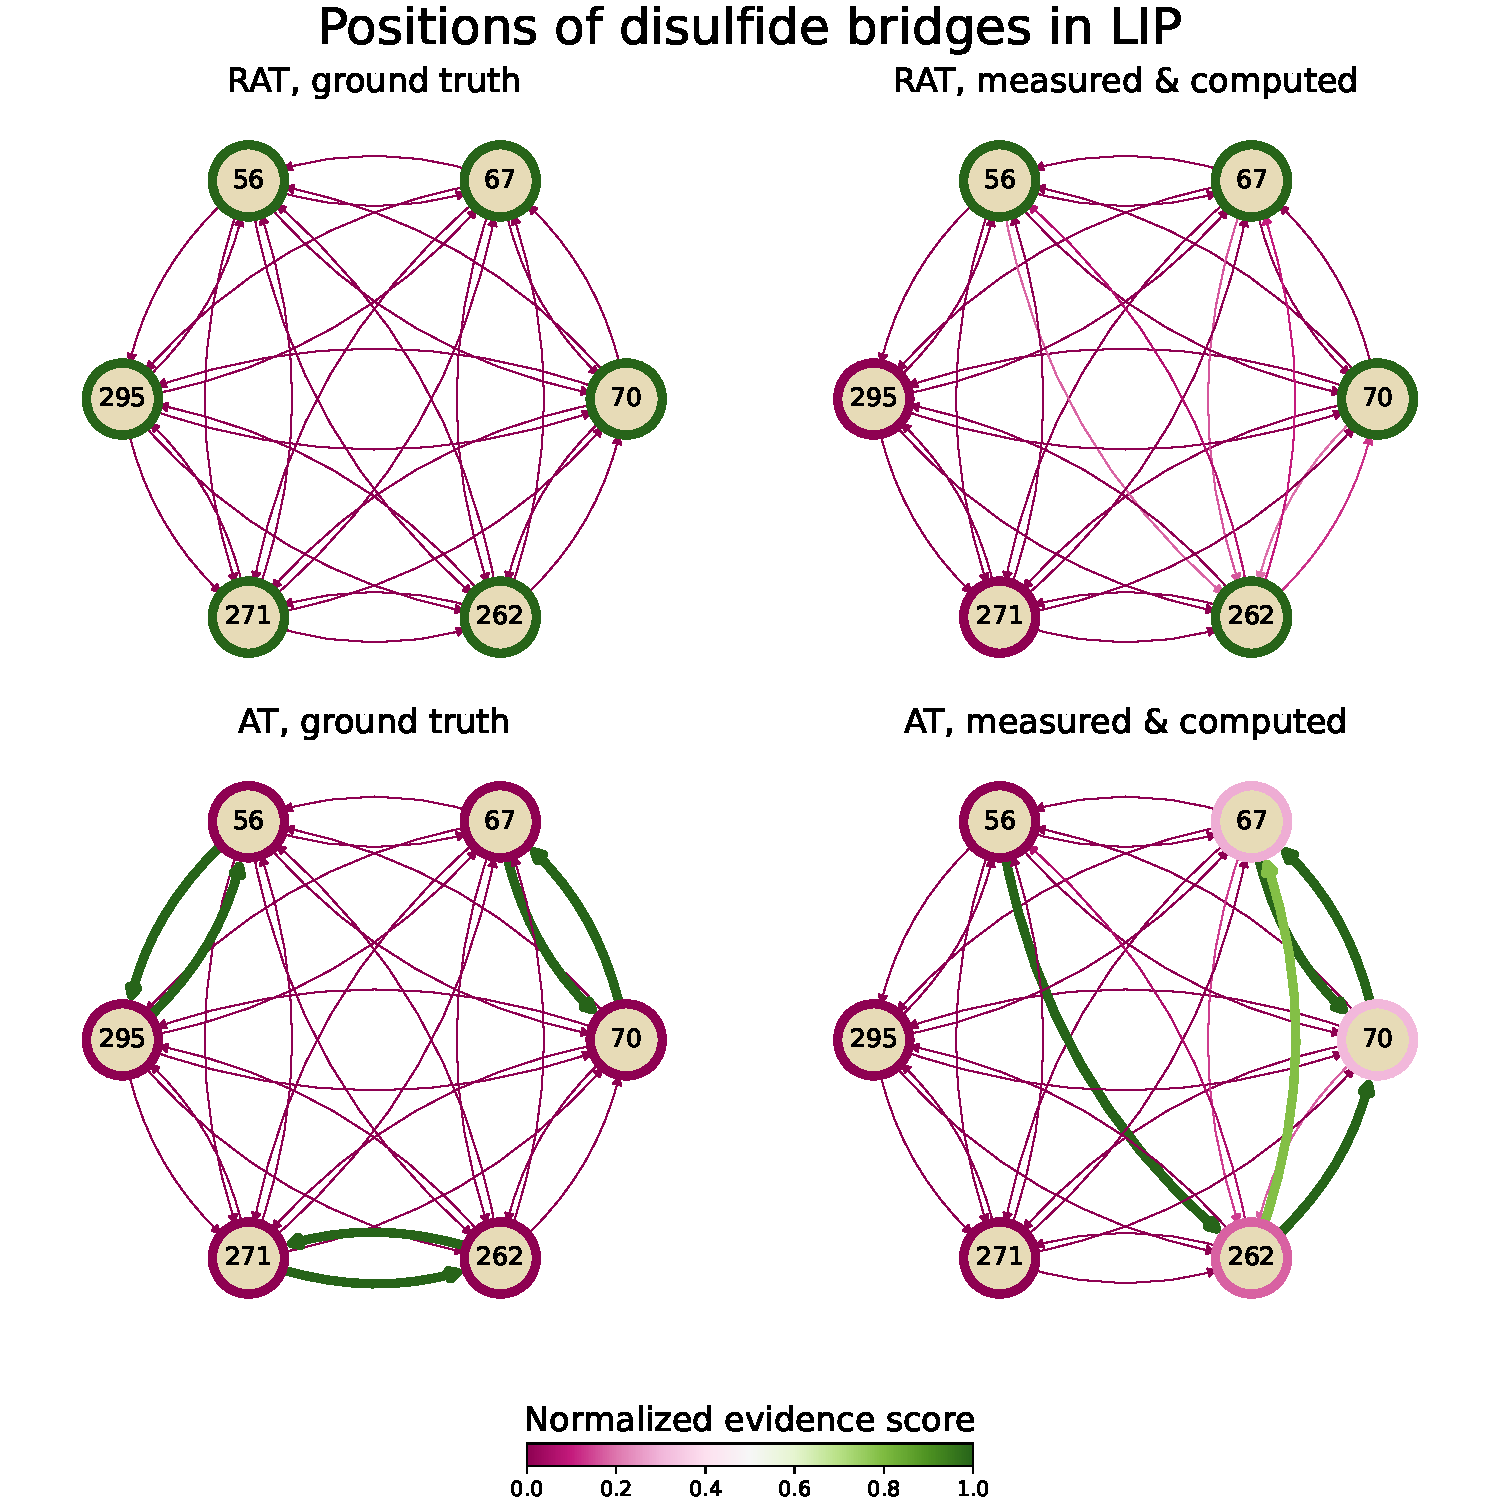
\includegraphics[width=1\linewidth]{img/lip.pdf}
  \caption{The evidence for positions of DBs and alkylations in in-silico generated ovalbumin, weighted by variant score, and normalised. No fragments containing cysteines 271 and 295 have been assigned (neither in alkylated form, nor as a part of any disulfide bond); this leads us to believe that a part of the data has been lost, or otherwise damaged.}\label{fig:lip}
\end{figure}

To conclude, the scoring metric separates good variants from the bad ones rather well. With the help of the scoring system, Dibby managed to sift through the large number of false positive assignments, and successfully identified most of the true DBs in the LYS and GENOVA samples. One true DB has even been identified in LIP, despite the problems in the LIP dataset.


\section{Discussion}

It is impossible to directly test how well the scoring metric (\Cref{sec:scoring}) separates true positives from false positives, because we do not know which peaks were generated by which fragments. However, we do know where the DBs are located in the protein, in theory. We will call a fragment (and by extension, the whole variant) that contradicts our knowledge about DB position a \emph{bad} fragment. In order for the scoring metric to be useful, bad fragments and variants should in general have a lower score than good ones.  In order for the scoring metric to be useful, bad fragments and variants should in general have a lower score than good ones.

We have found that the metric in general satisfactorily spearates the ``good'' variants from the bad ones, nonetheless there are still many ``bad'' variants with a high score. In the in-silico generated GENOVA dataset the upper tail end of the bad variants ends much lower than it does in the other samples. We interpret this as follows: the upper part of the tail can be attributed to DB scrambling, a process that occured duting the preapartion of the real-world datasets, but didn't occur during the generation of GENOVA. In other words, the high-scoring bad variants should not exist in theory, but they were observed  in the data with great condifence, and scored appropriately. On the other hand, the lower end of the tail are probably false positives probably caused by imprefections in our matching and scoring system

%TODO Přidat lepší discussion, podle Mirka.

% \chapter{Results and discussion}

% \section{Graphics and figure quality}

% \subsection{Visualize all important ideas}
% The set of figures in your thesis should be comprehensive and complete. For all important ideas, constructions, complicated setups and results there should be a visualization that the reader can refer to in case the text does not paint the `mental image' sufficiently well. At the bare minimum, you should have at least 3 figures (roughly corresponding to the 3 chapters) that clearly and unambiguously show:

% \begin{enumerate}
%   \item the context of the problem you are solving, optionally with e.g.~question marks and exclamation marks placed to highlight the problems and research questions
%   \item the advancement or the distinctive property of your solution, usually in a benchmark plot, or as a clear demonstration and comparison of the results.
% \end{enumerate}

% \subsection{Make the figures comprehensible}
% The figures should be easily comprehensible. Surprisingly, that requires you to follow some common ``standards'' in figure design and processing. People are often used to a certain form of the visualizations, and (unless you have a very good reason) deviating from the standard is going to make the comprehension much more complicated. The common standards include the following:

% \section{What is a discussion?}
% After you present the results and show that your contributions work, it is important to \emph{interpret} them, showing what they mean for the more general public.

% Separate discussion sections are common in life sciences where ambiguity is common and intuition is sometimes the only thing that the authors have; exact sciences and mathematicians do not use them as often. Despite of that, it is nice to precisely set your output into the existing environment, answering:
% \begin{itemize}
%   \item What is the potential application of the result?
%   \item Does the result solve a problem that other people encountered?
%   \item Did the results point to any new (surprising) facts?
%   \item Why is the result important for your future work (or work of anyone other)?
%   \item Can the results be used to replace (and improve) anything that is used currently?
% \end{itemize}